% Ch2LiteratureReview.tex

\chapter[Literature review]{An overview of frog call classification}
\label{cha:cha2LiteratureReview}

This chapter reviews the extant literature on frog call classification using machine learning algorithms. To the best of our knowledge, no previous studies focus on frog call classification using MIML or ML learning. Therefore, this chapter will mainly review the SISL  classification of frog calls. For MIML and ML learning, some prior work on bird call classification is reviewed. This review mainly aims to give a quantitative and detailed analysis of related techniques for frog call classification. 
Then, several major challenges that have not been addressed in prior work are identified, and hence the advances in this thesis are necessary and significant. Detailed information of each part will be described in following sub-section.

\section{Overview}
Three parts play important roles in the performance of frog call classification: signal pre-processing, feature extraction, and classification. Figure~\ref{ch2:fig:flowchart} depicts the common structure of frog call classification.

\begin{figure*}[htb!]
\centering
    \begin{subfigure}[b]{\textwidth}
           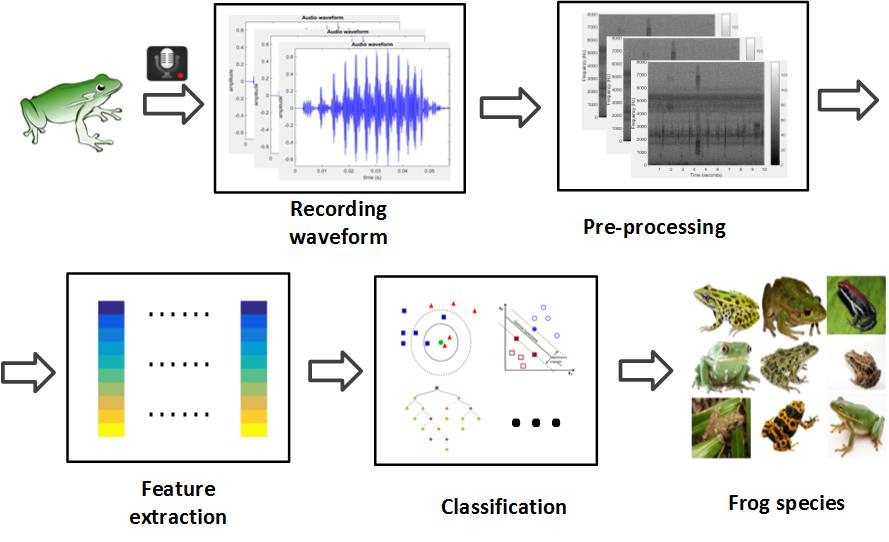
\includegraphics[width=\textwidth]{image/Ch1/flowchart.jpg}
    \end{subfigure}%
\caption{Flowchart of frog call classification: pre-processing, feature extraction, and classification.}
\label{ch2:fig:flowchart}       
\end{figure*}


%\section{Overview}
%\label{intro}
%Over the past decade, frog biodiversity has rapidly declined because of frogs' sensitivity to habitat loss and degradation, introduced invasive species, and environmental pollution \citep{dudgeon2006freshwater}. On the one hand, frog biodiversity is rapidly declining, and on the other hand frogs are greatly valuable to the environment. Firstly, frogs are an integral part of the food web, and the decline of their population can result in negative impacts through the whole ecosystem. Secondly, frogs are famous indicator species for environment health. Finally, frogs are very useful in medical research that benefits humans \footnote{http://www.savethefrogs.com/why-frogs}. The rapid biodiversity decline and great importance of frogs make it necessary for frog biodiversity monitoring to increase. 
%
%To monitor the change of frog biodiversity and optimise frog protection policies, many researchers have shown interest in studying frogs. Compared to counting frogs by visual observation, hearing the vocalisations of frogs is much easier. Consequently, frog vocalisations are often used for monitoring frogs. There are two approaches for acoustic frog monitoring. The traditional field survey methods require ecologists to physically visit sites to collect acoustic data, which is both time-consuming and costly. In contrast, recent advances in acoustic sensor techniques have greatly extended the spatio-temporal scale for acoustic monitoring of frog biodiversity \citep{wimmer2013analysing}. The large volumes of acoustic data collected this way make it essential to develop new automated methods of analysis. 
%
%
%Over the last few years, many researchers have described automated methods for detecting and classifying frog calls \citep{huang2008realization, huang2009frog, han2011acoustic,chen2012automatic, Gingras2013, camacho2013automatic, Huang20141}. However, there is no paper that summarises those methods. In this work, we present a comprehensive survey of frog call classification to provide other researchers with basic information, current methods and trends in this field. 
%
%Three parts play important roles in the performance and precision of frog call classification: signal pre-processing, feature extraction, and classification. In this survey, these three important parts of frog call classification are presented as shown in Figure~\ref{fig:Ch1_flowchart}. 
%
%
%
%
%Signal pre-processing consists of signal processing, noise reduction and syllable segmentation. Signal processing here denotes changing a signal from one-dimension (audio data) into two-dimensional representation (image). Noise reduction is essential to improve the classification performance. Since the elementary acoustic unit for frog call classification is the syllable, which is a continuous vocalisation emitted by an individual, segmenting continuous recordings of frog calls into individual syllables is necessary. 
%
%Previous studies have developed various methods for feature extraction \citep{huang2008realization, huang2009frog, han2011acoustic, chen2012automatic, Gingras2013, camacho2013automatic, Huang20141}. Here we review and analyse all the used features: time domain and frequency domain features, 
%time-frequency features, cepstral features, and other features. After feature extraction, numerous classifiers have been proposed for frog call classification. A summary of those classifiers is given in section \ref{classifiers}.
%
%
%It is worth noting that most previous researchers used different databases for their experiments because frog call research is often related to geographical regions \citep{jang2011geographic}. Consequently, there is still a lack of uniformity in the way classification methods are evaluated and assessed. This survey is not meant to compare all previous frog call classification methods and find the best one, but to assemble all the methods in order to provide a direction for the classification of frog calls. To be specific, this research mainly surveyed different features used for frog call classification because most studies focus on new features rather than new signal processing techniques, syllable segmentation methods, or classifiers.
%

%
%
%The remainder of this survey is organised as follows: In section \ref{pre-processing}, signal pre-processing is presented in its three parts: signal processing, noise reduction, and syllable segmentation. 
%In section \ref{features}, different acoustic features are investigated for frog call classification. In section \ref{classifiers}, numerous classifiers are studied for frog call classification. In section \ref{experiment}, experimental results of state-of-the-art research are discussed. Finally, section \ref{discussion} discusses research gaps and \ref{conclusion} sums up this chapter.

 


\section{Signal pre-processing}
\label{pre-processing}

%Frog recordings are often collected using a battery-powered acoustic sensor (stored in a weather proof metal box) with an external microphone. After signal acquisition, signal preprocessing is the first step for a frog call classification system.
Signal pre-processing often contains signal processing, noise reduction, and syllable segmentation. 


\subsection{Signal processing}
Signal processing often denotes the transformation of frog calls from one dimension (recording waveform) to two dimensions (time-frequency representation). Techniques used for frog signal processing contains STFT \citep{huang2009frog, Huang20141, Colonna20157367}, WPD \citep{yen2002automatic}, and DWT \citep{colonna2012feature}. STFT is the most widely used technique for its flexible implementation and better applicability. Given one frog call $x(n)$, its fast Fourier transform can be expressed as
\begin{equation}
X(k) = \sum_{n=0}^{L-1}x(n)w(n)e^{-j2 \pi kn/L}, 0 \leq k \leq L-1
\end{equation}
where $X(k)$ is the frequency domain signal (spectrum) and denotes each frame of the spectrogram, and $w(n)$ is the window function. The waveform, spectrum and spectrogram of one individual syllable for \textit{Mixophyes fasciolatus} is illustrated in Figure~\ref{fig:spectrogram}. 

\begin{figure*}[htb!]
\centering
      \begin{subfigure}[b]{0.32\textwidth}
           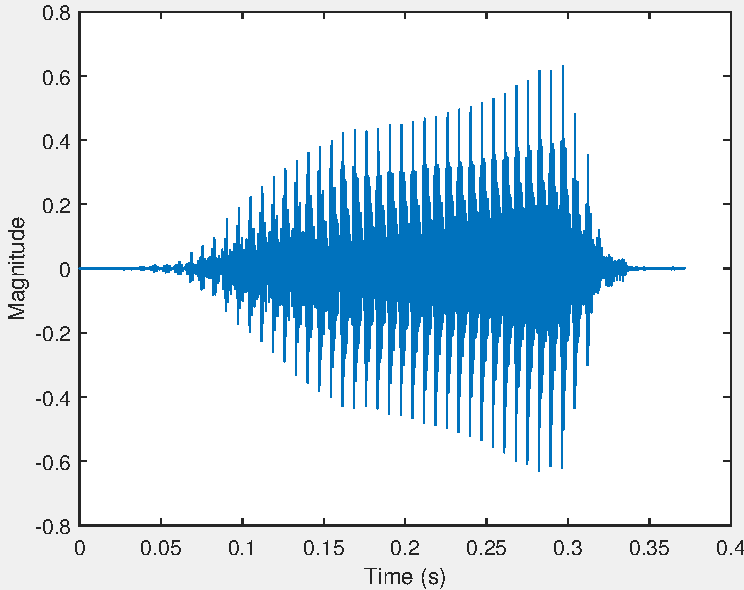
\includegraphics[width=1\textwidth,height=0.75\textwidth]{image/LR/waveform.pdf}
    \end{subfigure}%
	~
	      \begin{subfigure}[b]{0.32\textwidth}
           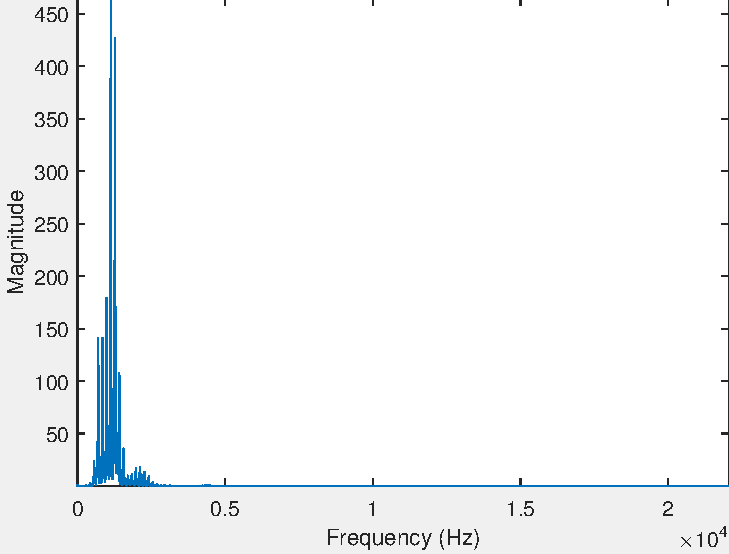
\includegraphics[width=1\textwidth,height=0.75\textwidth]{image/LR/spectrum.pdf}
    \end{subfigure}%
	~
    \begin{subfigure}[b]{0.32\textwidth}
           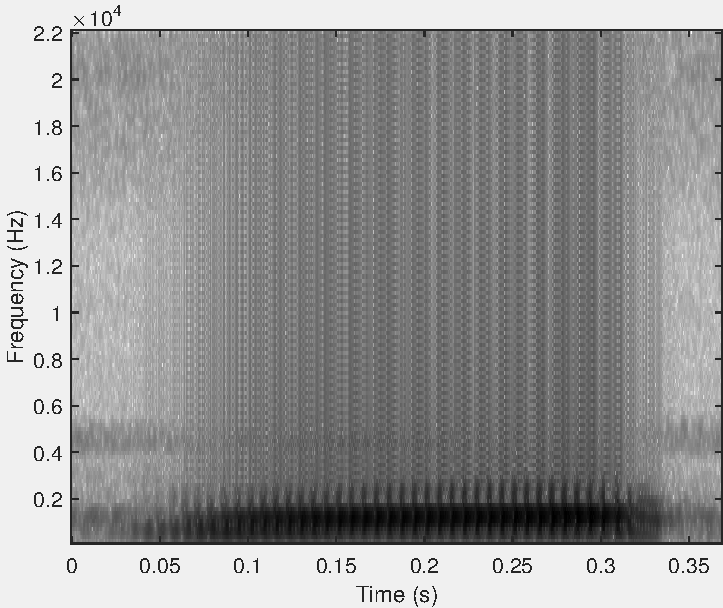
\includegraphics[width=1\textwidth,height=0.75\textwidth]{image/LR/spectrogram.pdf}
    \end{subfigure}%
\caption[Waveform, spectrum and spectrogram of one frog syllable]{Waveform, spectrum and spectrogram of one frog syllable for \textit{Mixophyes fasciolatus}. The window function, size and overlap are Hamming window, 128 samples and 85\%, respectively}
\label{fig:spectrogram}       % Give a unique label
\end{figure*}


%So far, wavelet packet decomposition (WPD) is the another technique that applied for frog call classification \citep{jie2015escience}. However, different from 

%Besides STFT, Xie et al recently introduced . 
%Compared with STFT, WPD has a better frequency resolution.


\subsection{Noise reduction}
Noise reduction is an optional process for frog call classification. 
\cite{Huang20141} applied a de-noise filter for noise reduction. A wavelet threshold function in the one-dimensional signal was used as the filter kernel function.
\cite{bedoya2014automatic} introduced a spectral noise gating method for noise reduction. Specifically, the selected frequency band spectrum of the frogs' call to be detected was estimated and suppressed. Although the aforementioned noise reduction methods can reduce the background noise, some of the desired signals will be suppressed. Noise reduction are thus selectively used based on the SNR of acoustic data and the research problem.




\subsection{Syllable segmentation}
For frog calls, the basic elementary acoustic unit is a syllable, which is a continuous frog vocalisation emitted by an individual frog \citep{huang2009frog}. The accuracy of syllable segmentation will directly affect the classification performance, because features for frog call classification are calculated from each segmented syllable. Frog syllable segmentation methods in previous studies are summarised and listed in Table~\ref{tab:segmentation}. However, all previous methods cannot address recordings with multiple simultaneously vocalising frog species. Meanwhile, those methods, which use temporal features for segmentation, cannot address low SNR recordings. 

%\cite{jie2015ICIP} introduced an unsupervised learning method, which included multiple image processing techniques for syllable segmentation. However, the downside of this unsupervised process was that not all segmented syllables correspond to frog vocalisations.

%Since the accuracy of segmentation results directly affect the final classification accuracy \citep{Colonna20157367}, meanwhile we focus on the evaluation of different features for frog call classification in this survey, we manually segment the frog calls for reducing the effect of segmentation result for classification accuracy,
  
\begin{table}[htb!]
\centering
\caption[Summary of related work]{Summary of prior work for frog syllable segmentation. Here, \textit{E} denotes energy, \textit{ZCR} denotes zero-crossing rate. Sequential means that syllables are segmented using the same sequence of those syllables in the recording.}
\label{tab:segmentation}
\resizebox{\textwidth}{!}{
\begin{tabular}{lll}
\hline\hline
{\bf Authors} & {\bf Features for segmentation}                    & {\bf Procedure}                          \\ \hline
   \citet{han2011acoustic}            & Spectral entropy                  & Manual                                      \\ 
  \citet{jaafar2013mfcc}             & E and ZCR                         & Sequential                \\ 
    \citet{huang2009frog}           & Amplitude                         & Non-sequential                           \\ 
    \citet{harma2003automatic}           & Spectrogram                          & Non-sequential           \\ 
     \citet{Colonna20157367}          & Incremental E and Incremental ZCR & Sequential and real time      \\
    % \citet{jie2015ICIP}   &    Image processing    & Non-sequential    \\    
      \hline\hline
\end{tabular}
}
\end{table}




\section{Acoustic features for frog call classification}
\label{features}
Developing effective acoustic features that show greater variation between rather than within species is important for achieving a high classification performance \citep{Fox20081187}. For frog call classification, acoustic features can be classified into five categories: temporal features, perceptual features, time-frequency features, cepstral features, and other features. 

\subsection{Temporal and perceptual features for frog call classification}

Temporal features for frog call classification have been explored for a long time \citep{huang2008realization, huang2009frog, dayou2011classification, chen2012automatic, camacho2013automatic, Huang20141}. To achieve a better classification performance, temporal features are often combined with perceptual features for frog call classification.
 
\cite{huang2009frog} used spectral centroid, signal bandwidth, and threshold-crossing rate for frog call classification with kNN and SVM. In another work, \cite{Huang20141} combined spectral centroid, signal bandwidth, spectral roll-off, threshold-crossing rate, spectral flatness, and average energy to classify frog calls using NN. Another paper published by  \citep{huang2008realization} used spectral centroid, signal bandwidth, spectral roll-off, and threshold-crossing rate for frog call classification. 
\cite{dayou2011classification} combined Shannon entropy, R$\acute{e}$nyi entropy and Tsallis entropy for frog call classification. Based on this work, \cite{han2011acoustic} improved the classification accuracy by replacing Tsallis entropy with spectral centroid.
To classify anurans into four genera, a three-parameter model was proposed based on advertisement calls\footnote[1]{an advertisement call is produced by a male frog in order to attract females during the breeding season and to warn other rival males of his presence.}, which used mean values for dominant frequency, coefficients of variation of root-mean square energy, and spectral flux \citep{Gingras2013}. With this model, three classifiers  were employed for classification: kNN, a multivariate Gaussian distribution model and GMM \citep{Gingras2013}.
\cite{chen2012automatic} proposed a method based on syllable duration and a multi-stage average spectrum for frog call recognition. Their recognition stage was completed by the Euclidean distance-based similarity measure. \cite{camacho2013automatic} used the loudness, timbre and pitch to detect frogs with a multivariate ANOVA test.






\subsection{Time-frequency features for frog call classification}

For frog call classification, one-dimensional recording waveform is often transformed into its two-dimensional time-frequency representation. Then, features based on the time-frequency representation are computed for classification.
\cite{acevedo2009automated} developed two feature sets for automated animal classification. The first was minimum and maximum frequencies, call duration, and maximum power; the second was minimum and maximum frequencies, call duration, and frequency of maximum power in eight segments of duration. With two feature sets, three classifiers were used for the classification: LDA, DT, and SVM. \cite{brandes2008feature} proposed a method for classifying animal calls using duration, maximum frequency, and frequency bandwidth, and with HMM used as the classifier. \cite{yen2002automatic} combined wavelet transform and two different dimensionality reduction algorithms to produce the final feature. Then, a NN classifier is used for frog call classification. \cite{grigg1996monitoring} developed a system to monitor the effect of the introduced Cane Toad on the frog population of Queensland. The classification was based on the local peaks in the spectrogram using Quinlan's machine learning system, C4.5. \cite{Brandes2006} proposed a method to classify frogs using central frequency, duration, and bandwidth with a Bayesian classifier. \cite{croker2012using} introduced a novel feature set for detecting frogs with a similarity measure based on Euclidean distance. The feature set contained dominant frequency, frequency difference between the lowest and dominant frequencies, frequency difference between the highest and dominant frequencies, time from the start of the sound to the peak volume, and time from the peak volume to the end of the sound. 
 


\subsection{Cepstral features for frog call classification}

Cepstral features (MFCCs) are popular for frog call classification. 
 \cite{jaafarcomparative} introduced MFCCs and LPCs as features. Then kNN and SVM were used as classifiers for frog call identification. \cite{yuan2012frog} also used MFCCs and LPCs as features. Then kNN was used as the classifier for frog sound identification.
\cite{lee2006automatic} used the averaged MFCCs and LDA for the automatic recognition of animal sounds. \cite{bedoya2014automatic} combined MFCCs and LAMDA for frog call recognition. \cite{vaca2010using} proposed a method to identify animal species, which consisted of MFCCs, PCA and kNN. \cite{jaafar2013mfcc, tanintelligent2014} published three papers about frog call classification using MFCCs, $\Delta$ MFCC and $\Delta \Delta$ MFCC calculated as features. Then kNN and SVM were used for classification. \cite{feature2012Colona} introduced MFCCs for classifying anurans with kNN. 


\subsection{Other features for frog call classification}
Besides temporal features, perceptual features, time-frequency features, and cepstral features, other features are introduced to classify frog calls.
\cite{wei2012distributed} proposed a distributed sparse approximation method based on $\ell 1$ minimization for frog call classification.  \cite{dang2008lightweight} extracted the vocalisation waveform envelope as features, then classified calls by matching the extracted envelope with the original signal envelope. \cite{kular2015classifying} treated the sound signal of a frog call as a texture image. Then, texture visual words and MFCCs were calculated for frog call classification. 


%\begin{figure}[htb!]
%\centering
%      \begin{subfigure}[b]{0.5\textwidth}
%           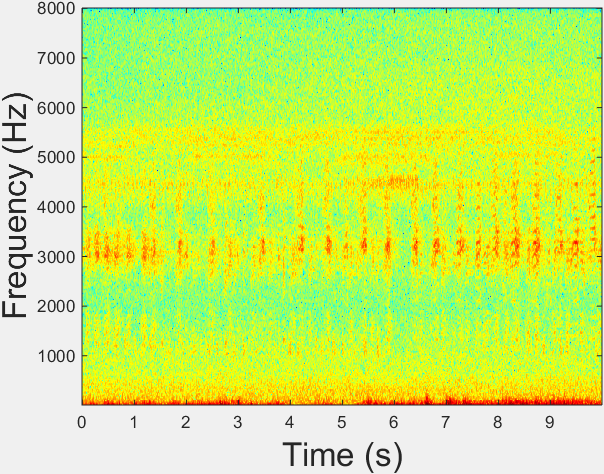
\includegraphics[width=1\textwidth,height=0.75\textwidth]{image/LR/spectrogram.png}
%    \end{subfigure}%
%	~~
%	      \begin{subfigure}[b]{0.5\textwidth}
%           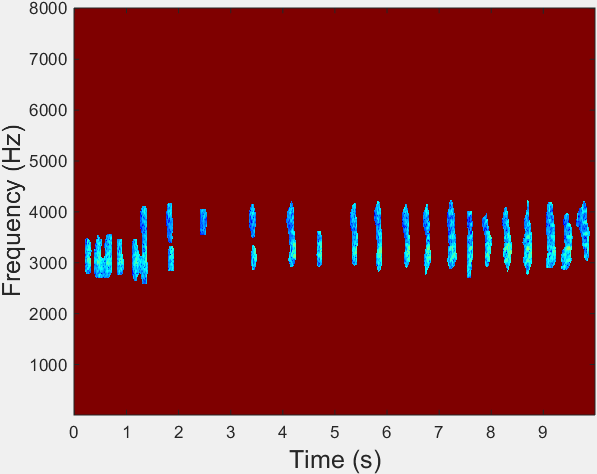
\includegraphics[width=1\textwidth,height=0.75\textwidth]{image/LR/segmentEvents.png}
%    \end{subfigure}%
%\caption[Acoustic event detection]{Original spectrogram and segmented events after applying acoustic event detection to the original spectrogram image.}
%\label{fig:evenets}       % Give a unique label
%\end{figure}



\section{Classifiers}
\label{classifiers}
For frog call classification, numerous pattern recognition methods have been used to construct the classifier, such as Bayesian classifier \citep{Brandes2006}, kNN \citep{ huang2008realization,huang2009frog, han2011acoustic, dayou2011classification, jaafar2013mfcc, Gingras2013, jaafar2013mfcc,jaafarcomparative, yuan2012frog, vaca2010using, feature2012Colona}, SVM \citep{huang2008realization,acevedo2009automated, huang2009frog, tanintelligent2014, Gingras2013,jaafarcomparative}, HMM \citep{brandes2008feature}, GMM \citep{huang2008realization, Gingras2013}, NN \citep{Huang20141, yen2002automatic}, DT \citep{grigg1996monitoring, acevedo2009automated}, one-way multivariate ANOVA \citep{camacho2013automatic}, and LDA \citep{acevedo2009automated,lee2006automatic}. Besides classifiers, other methods for classifying frog species included those based on the similarity measure \citep{croker2012using, dang2008lightweight, chen2012automatic} and those based on the clustering technique \citep{colombia2009frogs, wei2012distributed, bedoya2014automatic}. The summary of classifiers for frog call classification is listed in Table~\ref{tab:classifierscomp}.
kNN is the most commonly used classifier for its simplicity and easy application. However, kNN is sensitive to the local structure of the data, as well as to the distance and distance function. Therefore, kNN is often run multiple times based on different initial points. 
SVM is another widely used classifier for its good generalisation ability. However, the performance of SVM is quite sensitive to the selection of the regularisation and kernel parameters, and it is possible to over-fit when tuning these hyper-parameters. Since selecting suitable parameters for SVM is very important, most previous studies conducted the parameter setting by grid search  \citep{hsu2003practical}.

\begin{table}[htb!]
\centering
\caption{A brief summary of classifiers in the literature.}
\label{tab:classifierscomp}
\resizebox{\textwidth}{!}{
\begin{tabular}{llll}
\hline\hline
Reference                         & Classifier             & Reference                      & Classifier                   \\ \hline
\citet{Brandes2006}             & Bayesian classifier    & \citet{acevedo2009automated} & Support vector machine       \\ 
\citet{huang2008realization}    & K-nearest neighbour    & \citet{huang2009frog}        & Support vector machine       \\ 
\citet{huang2009frog}           & K-nearest neighbour    & \citet{tanintelligent2014}   & Support vector machine       \\ 
\citet{vaca2010using}         & K-nearest neighbour    & \citet{Gingras2013}          & Support vector machine       \\ 
\citet{dayou2011classification} & K-nearest neighbour    & \citet{jaafarcomparative}    & Support vector machine       \\ 
\citet{han2011acoustic}              & K-nearest neighbour    & \citet{jie2015ICIP}          & Support vector machine       \\ 
\citet{Gingras2013}             & K-nearest neighbour    & \citet{brandes2008feature}   & Hidden Markov model          \\ 
\citet{jaafar2013mfcc}          & K-nearest neighbour    & \citet{huang2008realization} & Gaussian mixture model       \\ 
\citet{jaafarcomparative}       & K-nearest neighbour    & \citet{Gingras2013}          & Gaussian mixture model       \\ 
\citet{yuan2013frog}            & K-nearest neighbour    & \citet{Huang20141}           & Neural networks              \\ 
\citet{jaafar2013}           & K-nearest neighbour    & \citet{yen2002automatic}     & Neural networks              \\ 
\citet{Xie1504:Acoustic}        & K-nearest neighbour    & \citet{grigg1996monitoring}  & Decision tree                \\ 
\citet{emr2015Xie}              & K-nearest neighbour    & \citet{acevedo2009automated} & Decision tree                \\ 
\citet{jie2015escience}         & K-nearest neighbour    & \citet{camacho2013automatic} & One-way multivariate ANOVA   \\ 
\citet{feature2012Colona}       & K-nearest neighbour    & \citet{acevedo2009automated} & Linear discriminant analysis \\ 
\citet{huang2008realization}    & Support vector machine & \citet{lee2006automatic}     & Linear discriminant analysis \\ \hline\hline
\end{tabular}
}
\end{table}

\section{MIML or ML learning for bioacoustic signal classification}
To the best of this author's knowledge, there is still no paper that uses MIML or ML learning to focus on frog call classification. In contrast, some previous research has applied MIML or ML learning to study bird calls.

For MIML learning, \citet{briggs2012acoustic} introduced the MIML classifiers for acoustic classification of multiple simultaneously vocalising bird species. In their method, a supervised learning classifier (RF) was first employed for segmenting acoustic events. Then features were extracted from each segmented acoustic event. Before putting features into classifiers, a bag generator was used to construct a bag-level feature. Lastly, three MIML classifiers were experimentally evaluated: MIML-SVM, MIML-RBF, and MIML-kNN.
\citet{dufour2013multi} used MFCCs and three MIML classifiers to classify birds. To be specific, MFCCs were first calculated for each frame. Then two new feature vectors were computed to represent longer segments.
Lastly, three MIML classifiers were experimentally evaluated: MIML-RBF, MIML-kNN, and M3MIML (Maximum Margin Method for Multi-instance Multi-label Learning). 

For ML learning, several papers have been published in the Neural Information Processing Scaled for Bioacoustics (NIPS4B challenge), which classified birds, insects, and amphibians recordings, followed by pre-processing and segmentation, feature extraction, feature selection, and classification \citep{lasseck2013bird, stowell2013feature, mencia2013learning, massaronensemble, chen2013novel}. \citet{lasseck2013bird} first processed the recordings via the application of STFT, noise reduction and segmentation. Then, file-statistics, segment-statistics and segment-probabilities were calculated as  features. Finally, an ensemble of randomised decision trees was used for the classification of each sound class. \citet{stowell2013feature} used either MFCC statistics (52 dimensions), chirplet histograms (up to 20,000 dimensions), or both, as  features. Then, RF was used for ML classification. \citep{mencia2013learning} proposed a new feature extraction method via an unsupervised generation of an aleatory number of features, which included random patching, a de-noising auto-encoder unit and subsequent convolution. For the classification, a pairwise ensemble of SVMs, random decision trees and a single layer NN were used. \citet{massaronensemble} described an approach that involved building an ensemble of generalised linear models and a classification model by hinge loss and program based on stochastic gradient descent optimisation, and boosted trees ensembles. 
\citet{chen2013novel} first calculated prominent features from windowed MFCCs, and leveraged them to build an ensemble classifier which was a blend of different classifiers (Gradient Boosting Tree models, RF, Lasso and elastic-net regularized generalised linear model).




\section{Experiment results of state-of-the-art frog call classification}
\label{ch2:experiment}


\subsection{Evaluation criteria}

Accuracy is the most widely used statistical criterion for evaluating frog call classification. Other evaluation criteria such as precision, recall, sensitivity, specificity, F-measure, and ROC curves are also used. Before defining these evaluation criteria, we first define true positives (TP), true negatives (TN), false negatives (FN), and false positives (FP) as described by  \citep{gordon2003sequence} 
(1) TP: correctly recognised positives;
(2) TN: correctly recognised negatives;
(3) FN: positives recognised as negatives;
(4) FP: negatives recognised as positives.
Then, accuracy, precision, recall (sensitivity), specificity, and false positive rate can be defined as

\begin{equation}
Accuracy = \frac{TP+TN}{TP+TN+FP+FN}
\end{equation}

\begin{equation}
Precision = \frac{TP}{TP+FP}
\end{equation}

\begin{equation}
Recall = \frac{TP}{TP+FN}
\end{equation}

\begin{equation}
Specificity = \frac{TN}{FP+TN}
\end{equation}

\begin{equation}
FPR = \frac{FP}{FP+TN}
\end{equation}

\subsection{Previous experimental results}


Table~\ref{tab:classificationPerformance} shows the list of summarised frog call classification methods, together with the database they used and corresponding performance. From~Table \ref{tab:classificationPerformance}, we can find that few studies explored frog vocalisations using signal processing and machine learning techniques before 2010. Due to the decrease of frog biodiversity, advances in signal processing, machine learning techniques and acoustic sensors, the research in frogs has been increased in the last five years. In addition, few datasets are publicly shared with researchers. The classification performance of different studies varies a lot. One of the main reasons is the use of different datasets. 



\begin{table}[p]
\centering
\caption{A brief overview of frog call classification performance.}
\label{tab:classificationPerformance}
\resizebox{\textwidth}{!}{
\Rotatebox{90}{%
\begin{tabular}{llll}
\hline\hline
\textbf{Database}                   & \textbf{Performance}                   & \textbf{Reference} & \textbf{Data source} \\ \hline

22 frog species &  NA  & \citet{grigg1996monitoring} & Collected from Queensland, Australia (unavailable) \\ 

4 frog species with 66 samples & \begin{tabular}[c]{@{}l@{}}  Best performance with averaged classification \\ Accuracy of 72.18\% and 0.76\% for standard \\ deviation.  \end{tabular}  &  \citet{yen2002automatic} & Unknown \\

17 animal types & \begin{tabular}[c]{@{}l@{}}  50\% true positive accuracy, \\ over 50\ false-negative for 4 animal types \end{tabular}  & \citet{Brandes2006} & Collected from NE Costa Rica (unavailable) 
\\  


30 frog species and 19 cricket calls  &  \begin{tabular}[c]{@{}l@{}}  Averaged classification accuracy of 96.8\% \\ and 98.1\% \end{tabular}  & \citet{lee2006automatic}*  & Derived from compact disk (unavailable) \\ 

3 frog species with 50 samples &  Averaged  classification accuracy of 90\%       &           \citet{dang2008lightweight} & Unknown \\

5 frog species with 727 syllables & Averaged classification accuracy of 95.86\%     &   \citet{huang2008realization}  & Unknown  \\ 

\begin{tabular}[c]{@{}l@{}} 10 frog species, 9 bird species, \\ and 8 cricket species \end{tabular} & Accuracy of 88\% for frogs    & \citet{brandes2008feature}* & Collected from NE Costa Rica (unavailable) \\ 

\begin{tabular}[c]{@{}l@{}} 9 frog species and 3 bird species \\ with 10061 samples \end{tabular} & \begin{tabular}[c]{@{}l@{}} Best true positive rate of 94.95\% and \\ 0.94\% for false positive rate \end{tabular} &  \citet{acevedo2009automated}* &   Collected from 14 montane sites in Puerto Rico
 \\  
 
5 frog species with 959 samples      &   Averaged classification accuracy of 90.03\%       &    \citet{huang2009frog}  &   Unknown        \\  
 
\begin{tabular}[c]{@{}l@{}} 12 frog species with 379 samples,  \end{tabular}  \\ 10 bird species with 193 samples &  Averaged classification accuracy of 86.6\%    &   \citet{vaca2010using}* &   \begin{tabular}[c]{@{}l@{}} Recorded in Puerto Rico  (http://www.amazon.com/Los\\-Anfibios-Reptiles-Puerto-Rico/dp/084770243X) (available) \end{tabular} 
 \\  
 
 
9 frog species with 90 syllables &  Averaged classification accuracy of 90.00\%      &  \citet{dayou2011classification}  &   Obtained from http://www.Frogsaustralia.
net.au/frogs \\  
 
 
  9 frog species with 54 syllables   & Averaged classification accuracy of 98.00\%  &   \citet{han2011acoustic} &   Obtained from http://www.Frogsaustralia.
net.au/frogs \\  
 
1 frog species with 100 samples   & \begin{tabular}[c]{@{}l@{}}Sensitivity of 0.85 with specificity of 0.92  \\ when distinguishing \textit{Mixophyes iteratus} calls from \\ other species' call. Sensitivity of 0.88 with \\ specificity   of 0.82 against background noise \end{tabular}  & \citet{croker2012using} &  Recorded next to a running stream (unavailable) \\ 

  9 frog species with 49 samples            &    Averaged classification accuracy of 97.60\%  & \citet{feature2012Colona} &  \begin{tabular}[c]{@{}l@{}} Collected on the campus of the Federal
University of Amazonas in \\ Manaus, Brazil (unavailable) \end{tabular} 
\\ 

18 frog species with 960 syllables & Classification accuracy of 94.3\%   &   \citet{chen2012automatic} & \begin{tabular}[c]{@{}l@{}} Recorded in a wild field located in \\ the Shan-Ping forest ecological garden in Kaohsiung city, \\ Taiwan (unavailable) \end{tabular} \\ 

3 frog species with 635 calls & Precision of 99\%, recall of 92\% & \citet{camacho2013automatic} &  Collected from Costa Rica (unavailable)     \\ 


 142 species belonging to four genera   &  Genus classification accuracy above 70\%    &     \citet{Gingras2013} & obtained from
commercially available compact discs (CDs) (available)  \\ 

8 frog species with 160 samples & averaged classification accuracy of 98.1\%        &  \citet{yuan2013frog} &  Obtained from AmphibiaWeb (http://amphibiaweb.org/)(available)
\\ 
15 frog species with 386 syllables  &    Averaged classification accuracy of 85.78\%   &   \citet{jaafar2013mfcc} & Recorded from locations around Baling
and Kulim, Kedah, Malaysia (unavailable)
 \\ 

10 frog species with 250 syllables   &       Averaged classification accuracy of 98.8\%   &  \citet{jaafarcomparative} & \begin{tabular}[c]{@{}l@{}} Internet database (http://learning.froghome.org/) \\ and IBM,USM (http://www.frogwatch.org.au/?action=animal.list) (available) \end{tabular}  \\ 

12 frog species with 291 syllables &   Averaged classification accuracy of 97\%   & \citet{jaafar2013}  & Recorded from locations around Baling
and Kulim, Kedah, Malaysia (unavailable)
\\  

13 frog species with 1514 samples &  Averaged recognition rate of 93.4\%    &    \citet{Huang20141}  &   Unknown \\ 


15 frog species with 286 samples &       Averaged classification accuracy of 95.67\%   &  \citet{tanintelligent2014} & recorded at Sungai Sedim, in Kulim, Kedah, Malaysia   \\ 


13 frog species with 916 calls & \begin{tabular}[c]{@{}l@{}} Averaged classification accuracy of 100\%, \\ and 99.61\% respectively for two database \end{tabular}  &  \citet{bedoya2014automatic}  &  \begin{tabular}[c]{@{}l@{}} Provided
by the Smithsonian Tropical Research Institute (STRI) \\ and the Grupo Herpetológico de Antioquia (GHA) (unavailable) \end{tabular}   \\ 



15 frog species with 896 syllables   & Precision of 99.00\%  &   \citet{Colonna20157367} & Obtained from Internet(http://
bit.ly/1b8bvyE) (available)  \\ 

10 frog species with 516 syllables & Averaged classification accuracy of 97.45\%    & \citet{jie2015escience}  &  Collected from compact disk (http://www.naturesound.com.au/) (available) \\

  15 frog species with 436 syllables             &        Averaged classification accuracy of 74.73\%         &      \citet{jie2015ICIP}  &  Collected from compact disk (http://www.naturesound.com.au/) (available)  \\ 

16 frog species with 898 syllables    & Averaged classification accuracy of 90.5\%   &    \citet{Xie1504:Acoustic}  &  Collected from compact disk (http://www.naturesound.com.au/) (available)       \\ 
\\  
 \hline\hline
\end{tabular}
}
}
\end{table}





\section{Summary}
\label{discussion}

This chapter reviews three main parts of a frog call classification system: signal pre-processing, feature extraction, and classification. The review also points out the research gap in current literature as follows:

\subsection{Database}
One major problem for frog call classification is the lack of a universal database. The databases used in prior work are often related to geographical regions, because researchers from different countries focus on particular frog species in their specific area (Table \ref{tab:classificationPerformance}). Therefore, it is difficult for researchers to compare their particular classification methods. Current studies often focus on the study of limited number of frog species (less than 100), but the number of known amphibian species is above 7000. To reach a high quality resolution, there still is a long way to go.


\subsection{Signal pre-processing}
Currently, STFT is the most widely used technique for frog call classification. However, STFT has a trade-off between time and frequency resolution, which restricts the discriminability of features extracted from the spectrogram. 

Noise reduction is an optional processing step for frog call classification. For some databases used as shown in Table~\ref{tab:classificationPerformance}, frog recordings have a high SNR, where noise reduction is unnecessary. However, when studying recordings of low SNR, noise reduction is essential for improving the classification performance \citep{bedoya2014automatic, Huang20141}. After noise reduction, both the accuracy of syllable segmentation and feature extraction can be relatively improved.

Frog syllable segmentation based on energy and zero-crossing rate cannot address low SNR recordings. Meanwhile, this method cannot segment frog syllables in low SNR recordings with multiple frog species. Recent use of unsupervised learning algorithms opens a path for segmenting frog syllables in low SNR recordings with multiple frog species. However, like other unsupervised algorithms, this method has a disadvantage that not all segmented syllables are frog vocalisations \citep{potamitis2015unsupervised}. \citep{briggs2012acoustic} used a supervised RF for bird call segmentation. However, this method required lots of tagged acoustic data to train the classifier.

For syllable segmentation, temporal features are more sensitive to  the background noise than perceptual features, because different frequency components can be separated by transforming the signal from temporal domain to perceptual domain. However, temporal features cannot segment  frog syllables in low SNR recordings with multiple frog species, because temporal features have no ability to separate different frequency components. Compared to temporal features, the use of amplitude-frequency information provides a robust method to segment low SNR recordings. 




\subsection{Acoustic features}
Most previous studies directly transplant features developed for speech recognition to analyse frog calls, which might not be suitable. For example, MFCCs, which are based on the calculation of a non-linear Mel-scale filter-bank, are designed for studying speech. The Mel-scale is designed for the perceptual scale of pitches judged by human listeners. The frequency distribution might not be suitable for studying frogs. The direct use of speech features will therefore restrict classification performance. 

Most perceptual features are extracted by directly calculating the statistics over frames, which will loss the temporal information. To add the temporal information of the feature set, temporal features can be combined with perceptual features and cepstral features to achieve higher classification accuracy. Transforming audio data into its two-dimensional representation (such as a spectrogram) for quick visual analysis, has led to increasing attention being given to image processing techniques for automatically analysing animal calls. Image features derived from spectrograms are worth investigating for frog call classification. Sparse coding has been widely applied for feature extraction in other scaled bioacoustics studies \citep{glotin2013sparse, razik2015sparse}, which could be a potential direction for frog call classification.

\subsection{Classifiers}
Almost all previous studies assume that each recording has only one frog species, and then a SISL classification framework is adopted to classify frog calls. However, recent advances in acoustic sensor techniques have collected large volumes of acoustic data that have multiple simultaneously vocalising frog species, because different frog species tend to call together to make a frog chorus (Figure~\ref{fig:label}). Based on this attribute of frog call recordings, the classification problem can be naturally framed as a MIML classification or a ML classification problem rather than SISL classification. In previous studies, MIML and ML learning have been used to solve bioacoustic problems, but mainly focus on birds. 




In the following chapters, we aims to address the identified research gap. Four experiments are designed and organised in the manner outlined in Figure.~\ref{fig:mainchapters}.


\begin{figure}[htb!]
\centering
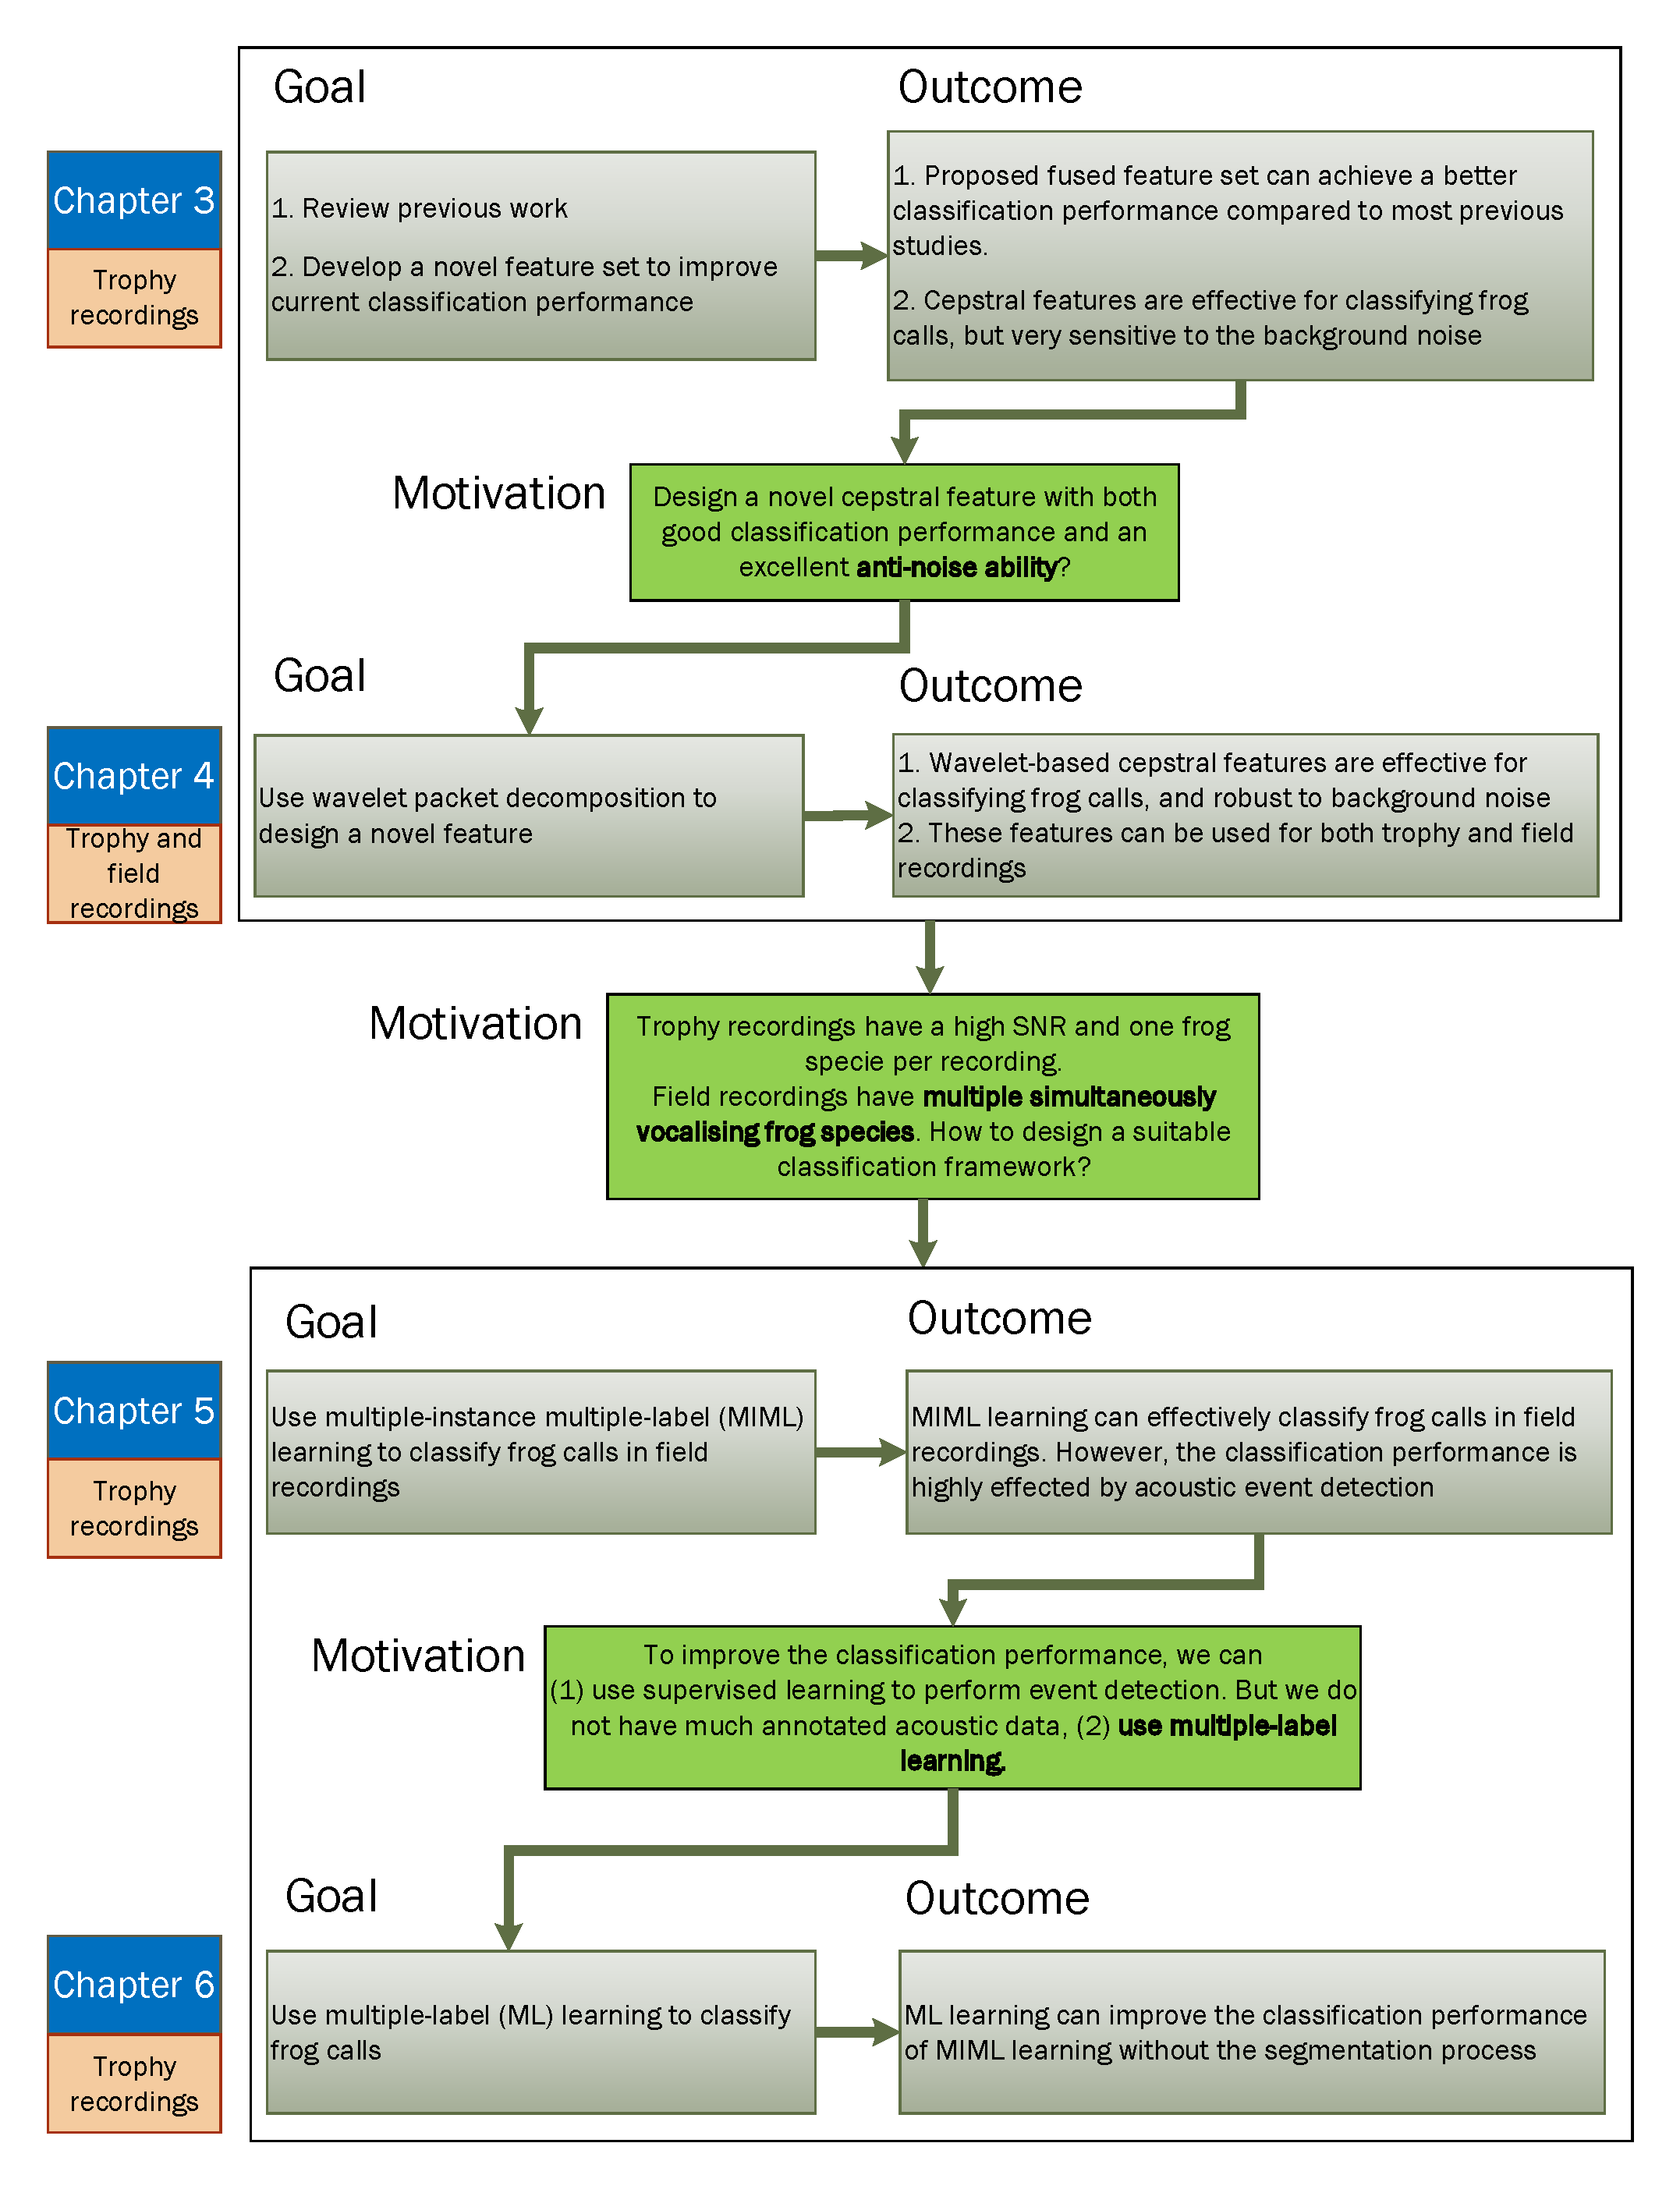
\includegraphics[width=\textwidth]{image/Ch1/structure_chapters.pdf}
\caption[Structure of the four main chapters of this thesis]{Structure of the four main chapters of this thesis}
\label{fig:mainchapters}
\end{figure}







%The main objective of this chapter is to provide a research direction for analysing frog calls. With the use of signal processing and machine learning techniques, different frog species can be classified based on their vocalisations. To achieve this goal, three main parts of a frog call classification system are reviewed: signal pre-processing, feature extraction, and classification. 

%For future work, it is worth further improving the accuracy and efficiency of noise reduction and syllable segmentation because they are critical processes for frog call classification. Since collected frog calls in the field often contain many background noises (birds, insects, rain, wind, human voices, etc.), it is necessary to design new noise reduction methods based on different environments. It is also necessary to develop accurate and efficient syllable segmentation methods for its great influence in the frog call classification system performance. Currently, studies have focused on frequency domain features for classification. In the future,  features extracted from various domains can be incorporated for increasing the frog call classification accuracy. For the classification framework, studying frog recordings with MIML learning or ML learning may be a productive research direction because of the attribute of collected environmental recordings. It is also worth making a uniform dataset that covers different frog species from different areas, since there is still no available uniform dataset of frog calls. Then researchers can evaluate their particular methods on a uniform platform.



%In general, frog call classification is still in its infancy as a field of study, and potential applications and unsolved problems are extending every day. 






